% !TeX spellcheck = de_DE
\documentclass{article}
\usepackage{cite}
\usepackage{amsmath,amssymb,amsfonts}
\usepackage{algorithmic}
\usepackage{graphicx}
\usepackage{float} 
\usepackage{subfigure}
\usepackage{textcomp}
\usepackage{xcolor}
\usepackage{booktabs}
\usepackage{caption}
\usepackage[colorlinks]{hyperref}
\usepackage{fontspec, xunicode, xltxtra}  
\usepackage{import}
\usepackage{ctex}
\usepackage{hyperref}
\usepackage{listings}
\usepackage{fontspec} % 定制字体
\newfontfamily\menlo{Menlo}
\usepackage{xcolor} % 定制颜色
\usepackage{underscore}
\definecolor{mygreen}{rgb}{0,0.6,0}
\definecolor{mygray}{rgb}{0.5,0.5,0.5}
\definecolor{mymauve}{rgb}{0.58,0,0.82}
\lstset{ %
	backgroundcolor=\color{white},      % choose the background color
	basicstyle=\footnotesize\ttfamily,  % size of fonts used for the code
	columns=fullflexible,
	tabsize=4,
	breaklines=true,               % automatic line breaking only at whitespace
	captionpos=b,                  % sets the caption-position to bottom
	commentstyle=\color{mygreen},  % comment style
	escapeinside={\%*}{*)},        % if you want to add LaTeX within your code
	keywordstyle=\color{blue},     % keyword style
	stringstyle=\color{mymauve}\ttfamily,  % string literal style
	frame=single,
	rulesepcolor=\color{red!20!green!20!blue!20},
	% identifierstyle=\color{red},
	language=matlab,
}
\usepackage{geometry}
\geometry{a4paper, scale=0.8}
\title{大作业报告}
\author{李文彬,1120173001}


\begin{document}
	


\section{K-means算法}
\subsection{算法简述}
K-means算法是一种迭代的、数值的、不确定的、无监督的聚类方法,它根据输入数据点之间的固有距离将它们分为多个类。K-means算法是基于数据成分对之间的相似性或相异性指数。
K-means算法假设数据特征形成一个向量空间,并试图在其中找到自然聚类。在这种方法中,像素点围绕聚类中心聚集,聚类中心则通过最小化空间获得的。\\K-means聚类是一种将图像的n个像素聚类成K个簇的技术,(K<n,K为正整数)。聚类中心在算法中是随机初始化的,聚类基于像素灰度强度和像素强度距离等相似性特征形成。
在这种聚类算法中,数据通过计算每个组的强度迭代地进行聚类,并通过用最接近的一个像素对类中的每个像素进行分类来分割图像。使用K-means算法分割图像要遵循的各个步骤如下:
\\将图像作为输入并计算强度分布。
\begin{itemize}
\item[1)]用k个随机强度初始化质心;
\item[2)]重复步骤,直到目标函数不再改变:
\item[3)]基于其强度与质心强度的距离对点进行聚类,
\item[4)]计算每个簇的新质心;
\end{itemize}
\subsubsection{更新公式}

聚类中心更新公式
$u_{i}=\frac{\prod_{j=1}^{N}P\left ( u_{i}|x_{j}\right )^{b}x_{j}}{\prod_{j=1}^{N}P\left ( u_{i}|x_{j}\right )^{b}}$ 
\subsubsection{算法规格}
\begin{itemize}
\item[1.]一个参数k,聚类中心的数目,当然也有一些常规的参数,比如最大迭代次数epochs,容忍度tol
\item[2.]一个循环,判断目标函数是否变化足够小,以F
范数(Frobenius norm)为度归


    
    \begin{lstlisting}
    
    while true,
    ...
    if norm(J_cur-J_prev, 'fro') < tol,
        break;
    end
    J_prev = J_cur;
end
    \end{lstlisting}
    
      \item[3.]一条更新语句,更新各个类的聚类中心,根据每个样本应属的类别(欧式距离最小表征)
    \begin{figure}[H]
        \centering
        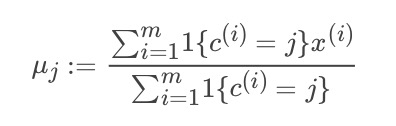
\includegraphics[width=0.4\textwidth]{img/al2.jpg} 
%        \caption{}

    \end{figure}
  
    \begin{lstlisting}
        dist = sum(X.^2, 2)*ones(1, k) + (sum(C.^2, 2)*ones(1, m*n))'...
        - 2*X*C';
    [~, idx] = min(dist, [], 2) ;
    for i = 1:k,
       C(i, :) = mean(X(idx == i , :)); % 即求解各集合中新的聚类中心
    end
    \end{lstlisting}
    \end{itemize}
\subsubsection{算法流程}
\begin{itemize}
\item[a] 初始化聚类个数k
\item[b] 循环,判断目标函数是否变化足够小,以F范式度量
\item[c] 推出循环,返回dist(到聚类中心距离矩阵),最新聚类中心,以及目标函数
\end{itemize}

\subsection{与Fuzzy C-Means算法比较}
硬聚类算法K-means相较于软聚类算法Fuzzy C-Means算法,更易快速迭代,达到全局最优;\\
Fuzzy C-Means虽然强调了各个样本和聚类中心的关系,但模糊隶属后更易受噪声干扰,因此更易陷入局部最优(因此对于Fuzzy C-Means的最基本优化方法是增加迭代次数);相较于Fuzzy C-Means,K-means逼近全局最优的资源消耗大幅下降,在本实验中表现优于Fuzzy C-Means算法;
\subsubsection{实验结果对比}
本实验中对于Kmeans算法中k值以及Fuzzy C-Means算法中k和b值进行了大量实验。\\
对于Kmeans,在k=19时可以达到最优分割效果,
而实验三中,Fuzzy C-Means在 k=19, b=4(k=19条件下,b=4时分割效果最好)时表现与K-means存在明显差距\\
对比结果如下
\begin{itemize}

\item[A.]K-means
绘制图像\\
 对最佳分割结果绘图
 
    \begin{figure}[H]
        \centering
        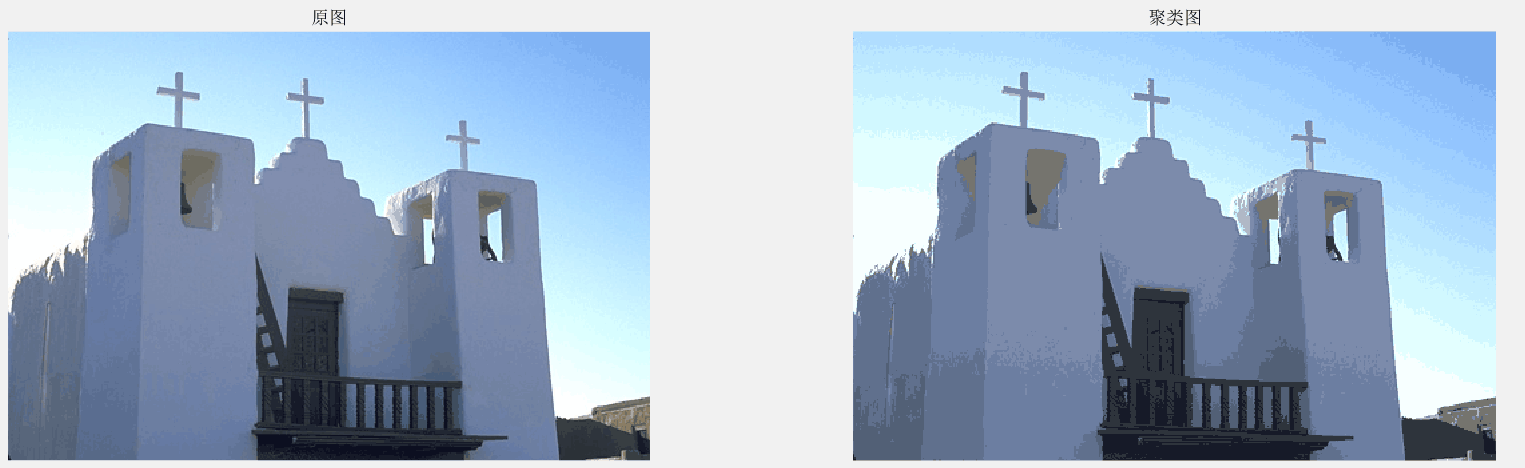
\includegraphics[width=0.9\textwidth]{img/K19.png} 
        \caption{原图像与分割后图像对比图}
        \label{fig.5}
    \end{figure}
   绘制函数迭代图
\begin{figure}[H]
	\centering
	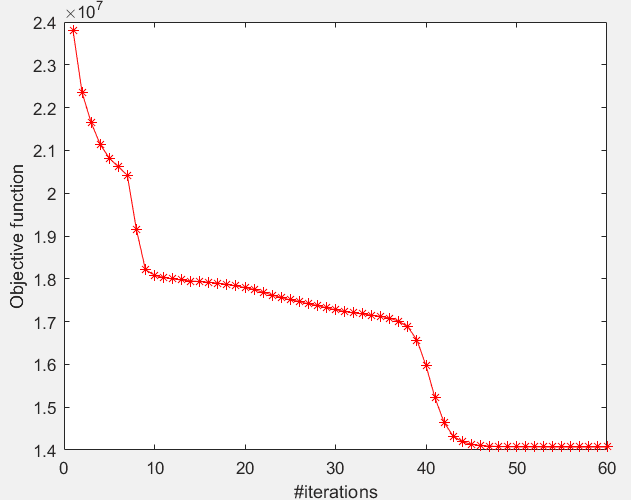
\includegraphics[width=0.6\textwidth]{img/funK19.png} 
	\caption{目标函数迭代结果}
	\label{fig.6}
\end{figure}   
\item[B.]对比Fuzzy C-Means\\
对K=19,b=2时分割效果绘图\\
观察分割后图像右上方渐变色天空可以看出,Fuzzy C-Means算法对于本图中渐变色的分割层次明显少于k值相同的K-means算法
 
    \begin{figure}[H]
        \centering
        \includegraphics[width=0.9\textwidth]{img/K15B4.png} 
        \caption{原图像与分割后图像对比图}
        \label{fig.7}
    \end{figure}
    
   绘制函数迭代图
\begin{figure}[H]
	\centering
	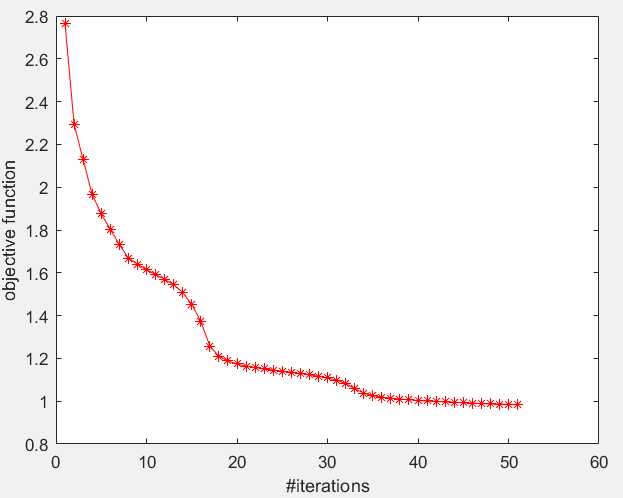
\includegraphics[width=0.6\textwidth]{img/funK15B4.png} 
	\caption{从两种算法中目标函数的迭代次数也可看出,K-means算法所需计算时间较少}
	\label{fig.8}
\end{figure}   
除以上对比外,Fuzzy C-Means 算法受 隶属度b值影响较大,在k取某些值时,经实验检测,b取值过大将造成分割效果较差或者目标函数不收敛的情况。
如, 在 k=15, b=6时,分割效果表现较差
\begin{figure}[H]
	\centering
	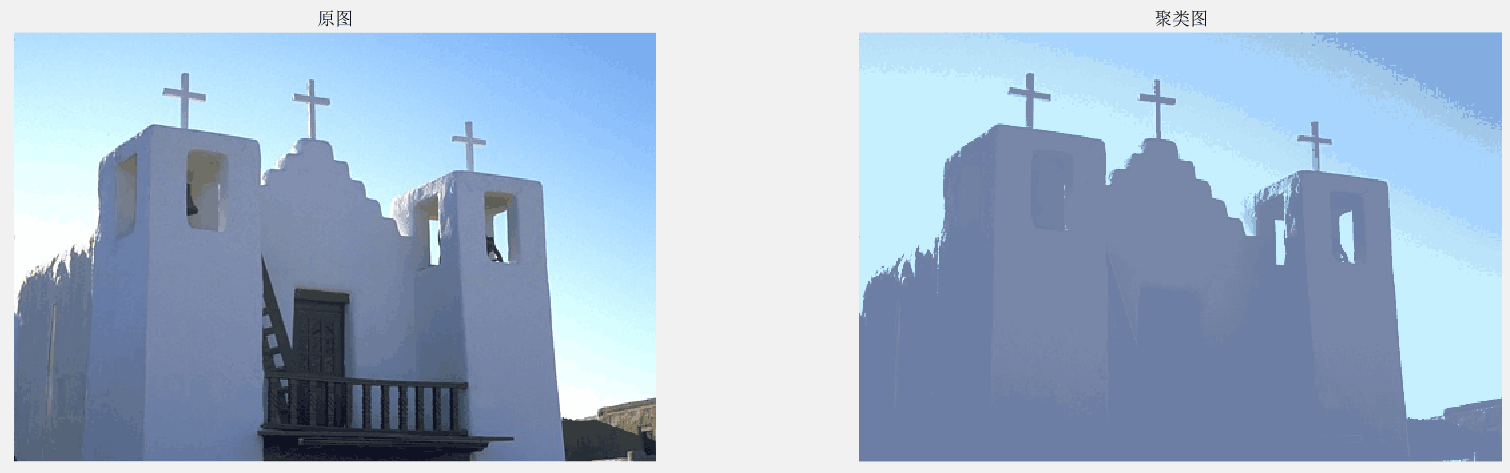
\includegraphics[width=0.6\textwidth]{img/K15B6.png} 
	\caption{目标函数迭代结果}
	\label{fig.2}
\end{figure}   
而在 k=15, b=4时,分割效果显著提高
\begin{figure}[H]
	\centering
	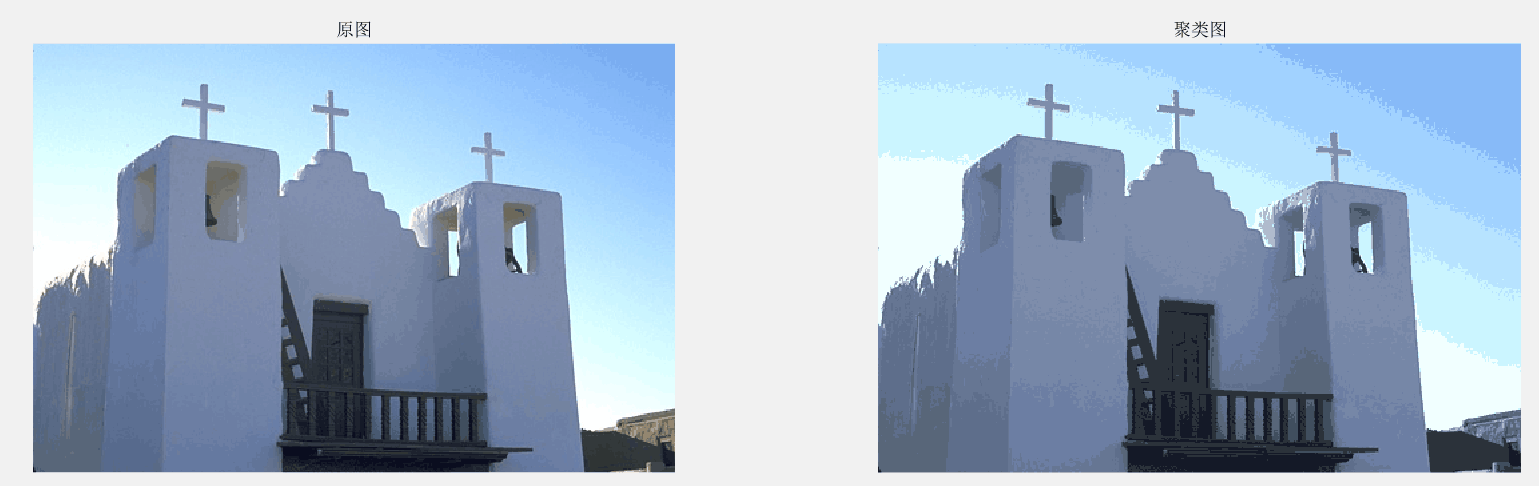
\includegraphics[width=0.6\textwidth]{img/K15B2.png} 
	\caption{目标函数迭代结果}
	\label{fig.8}
\end{figure}   
\end{itemize}
注 :\\
由于时间有限,本实验仅列出了最佳效果下的K-means分割图像以及目标函数,K-means和Fuzzy C-Means算法更多分割效果图详见文件夹imgKmeans和imgFCM
\subsection{主要功能实现相关代码展示}
\begin{lstlisting}
function [C, label, J] = kmeans(I, k)
[m, n, p] = size(I);
%将二维压缩成一维,转换精度
X = reshape(double(I), m*n, p);
rng('default');
%初始化聚类中心
C = X(randperm(m*n, k), :);
%初始化容忍度tol
J_prev = inf; iter = 0; J = []; tol = 1e-2;
%% 
%更新语句
while true
    iter = iter + 1;
    dist = sum(X.^2, 2)*ones(1, k) + (sum(C.^2, 2)*ones(1, m*n))' - 2*X*C';
    [~, label] = min(dist, [], 2) ;
    for i = 1:k
       C(i, :) = mean(X(label == i , :));
    end
    %计算目标函数
    J_cur = sum(sum((X - C(label, :)).^2, 2));
    J = [J, J_cur];
    fprintf('#iteration: %03d, objective function: %f\n', iter, J_cur);
    %判断目标函数变化是否足够小
    %F范数为度归
    if norm(J_cur-J_prev, 'fro') < tol
        break;
    end
    J_prev = J_cur;
end

\end{lstlisting}
 \section{补充说明}
 本实验所使用图片来源于UC-Berkely , Computer Vision Lab\\
 \href{https://www2.eecs.berkeley.edu/Research/Projects/CS/vision/grouping/resources.html}(https://www2.eecs.berkeley.edu/Research/Projects/CS/vision/grouping/resources.html)
\end{document}
